% Формализация задачи византийских генералов
\section{Формализация задачи византийских генералов}

\hspace{1.25cm}
Византия. Ночь перед великим сражением с противником. Византийская армия состоит из \(n\) легионов, каждый из которых командует свой генерал. Также у армии есть главнокомандующий, которому подчиняются генералы. В то же время империя находится в упадке, и любой из генералов, а также главнокомандующий, могут быть предателями, заинтересованными в её поражении.

Ночью каждый из генералов получает от предводителя приказ о варианте действий в 10 часов утра (время одинаковое для всех и известно заранее): «атаковать противника» или «отступать».

\underline{Возможные исходы сражения}

\begin{itemize}
    \item Если все верные генералы атакуют — Византия уничтожит противника (благоприятный исход).
    \item Если все верные генералы отступят — Византия сохранит свою армию (промежуточный исход).
    \item Если некоторые верные генералы атакуют, а некоторые отступят — противник уничтожит всю армию Византии (неблагоприятный исход).
\end{itemize}

Графически задача представлена на рисунке \ref{fig:byzantine}. 

\begin{figure}[h]
    \centering
    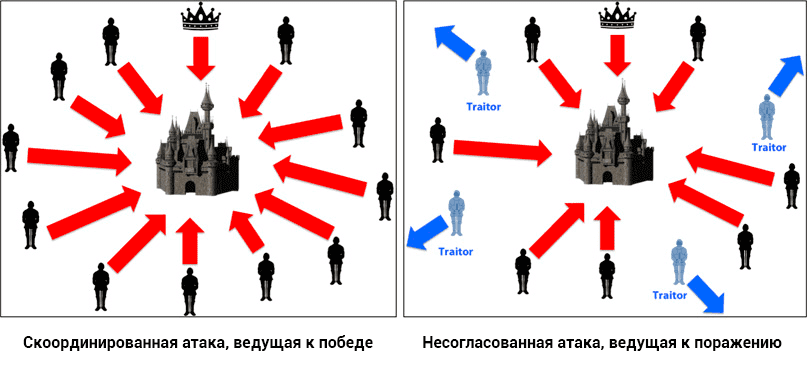
\includegraphics[width=\textwidth]{img/byzantine_generals.png} % Путь к вашему изображению
    \caption{Иллюстрация к «задаче византийских генералов»}
    \label{fig:byzantine}
\end{figure}

Также следует учитывать, что если главнокомандующий является предателем, он может дать разным генералам противоположные приказы, чтобы обеспечить уничтожение армии. Следовательно, генералам лучше не доверять его приказам. Если же каждый генерал будет действовать полностью независимо от других (например, сделает случайный выбор), то вероятность благоприятного исхода весьма низка. Поэтому генералы нуждаются в обмене информацией между собой, чтобы прийти к единому решению.~\cite{vakhramov}

\underline{Цель задачи:}

Найти алгоритм, который позволит лояльным генералам достичь консенсуса, несмотря на присутствие $m$ предателей, которые могут пытаться помешать принятию общего решения.

Задача византийских генералов является классической проблемой, моделирующей ситуации, где необходимо достичь согласия в условиях ненадежных участников и искажений информации.

\newpage